\documentclass[conference]{IEEEtran}
\IEEEoverridecommandlockouts

\usepackage{cite}
\usepackage{amsmath,amssymb,amsfonts}
\usepackage{graphicx}
\usepackage{textcomp}
\usepackage{xcolor}
\usepackage{booktabs}
\usepackage[hidelinks]{hyperref}

\begin{document}

\title{When the Faithfulness Metric Fails Before the Explanation Does:\\
Layer-wise Relevance Propagation on a Self-Supervised CT Foundation Model}

\author{\IEEEauthorblockN{Joana Owusu-Appiah}
\IEEEauthorblockA{\textit{Erasmus Mundus MSc Medical Imaging and Applications (MAIA)} \\
Girona, Spain \textbullet{} Dijon, France \textbullet{} Cassino, Italy \\
owusuappiahjoana59@gmail.com}}

\maketitle

\begin{abstract}
Attribution maps make a testable claim: the voxels they rank highest are the
ones the model used. Deletion metrics test that claim by masking top-ranked
voxels and watching the prediction fall. We apply this protocol to a
self-supervised CT foundation model, CT-FM, fine-tuned for lung-nodule
malignancy on volumetric chest CT, comparing three layer-wise relevance
propagation composites against Grad-CAM. Two findings follow. First, the
pretraining is worth having: CT-FM initialisation improves test AUC over an
architecturally identical randomly-initialised network at every label budget,
reaching 0.895 against 0.873 at full supervision, though a seed replicate shows
the smallest gain lies within seed noise. Second, and more consequentially,
\emph{no attribution method outperformed a random-order deletion baseline}. All
four scored worse, by 0.12 to 0.22 AOPC. We trace this to the baseline rather
than the explanations: random deletion scatters replaced voxels throughout the
volume and drives the input off the data manifold, whereas attribution-guided
deletion removes a compact contiguous region that remains far more plausible as
a scan. The random baseline wins by breaking the image, not by locating evidence
better. We report this as a failure of the metric under volumetric masking,
quantify the separation the methods do show under perturbation stability, where
Grad-CAM reaches 0.924 and LRP 0.012 to 0.220, and argue that deletion protocols
require manifold-preserving masking before they can adjudicate explanation
quality in 3D medical imaging.
\end{abstract}

\begin{IEEEkeywords}
explainable AI, layer-wise relevance propagation, foundation models,
self-supervised learning, uncertainty estimation, computed tomography
\end{IEEEkeywords}

\section{Introduction}

Two claims are commonly made in medical imaging papers and rarely tested
together. The first is that self-supervised pretraining on large unlabelled
image collections improves downstream performance. The second is that a
published attribution map explains the resulting model. Both are checkable, and
checking them is the subject of this paper.

We fine-tune CT-FM \cite{pai2025ctfm}, a SegResNet pretrained by contrastive
self-supervised learning on 148{,}000 CT scans, for benign-versus-malignant
lung-nodule classification on volumetric chest CT. We then explain it with
layer-wise relevance propagation (LRP) \cite{bach2015lrp} implemented in zennit
\cite{anders2021zennit}, whose layer-type registry covers \texttt{Conv3d} and
the 3D pooling operators and therefore applies to volumetric networks without
modification, and we benchmark LRP against Grad-CAM \cite{selvaraju2017gradcam},
the method most medical imaging work reaches for.

Our contributions are:

\begin{enumerate}
\item A label-efficiency ablation against an architecturally identical
      from-scratch control at 10\%, 25\% and 100\% of labels, with a seed
      replicate that identifies which gains survive.
\item A faithfulness evaluation of three LRP composites and Grad-CAM on 3D CT,
      reporting the negative result that none beats random-order deletion, with
      a diagnosis of why.
\item A measurement of explanation stability under input perturbation, which
      separates the methods where deletion does not, and an analysis of whether
      faithfulness degrades with predictive uncertainty.
\end{enumerate}

\section{Method}

\subsection{Data}

NoduleMNIST3D \cite{yang2023medmnist} comprises 3D chest CT patches centred on
lung nodules drawn from LIDC-IDRI \cite{armato2011lidc} and labelled benign or
malignant. Splits are 1{,}158 training, 165 validation and 310 test volumes,
with a 863:295 benign-to-malignant training imbalance. We therefore use
class-weighted cross-entropy, report balanced accuracy and AUC alongside
accuracy, and select models on validation AUC.

We use the $64^3$ release. This is not cosmetic: CT-FM downsamples by a factor
of 16, so a $28^3$ volume is not divisible by the network stride and raises an
error.

\subsection{Model and three silent failure modes}

CT-FM's encoder produces a five-level feature pyramid; we take the bottleneck at
512 channels and $4^3$ resolution, apply global average pooling, LayerNorm and a
linear head. Three implementation details are recorded because each fails
quietly and would have produced a plausible but meaningless result.

First, the published checkpoint does not load into MONAI's
\texttt{SegResNetDS}. Parameter names differ, and
\texttt{load\_state\_dict(strict=False)} matches \emph{zero of 161} tensors
without raising, so training proceeds on a randomly initialised network while
the code appears correct.

Second, the from-scratch control must be architecturally identical. Constructing
a second SegResNet from an inferred configuration yielded 19.9M parameters
against the true 87.2M; that ablation would have measured capacity and attributed
the difference to pretraining. Our control is the loaded model with every
parameter reinitialised.

Third, pooling the full SegResNet output rather than the bottleneck gives the
linear head two features. Combined with unnormalised activations, whose standard
deviation is approximately 0.03, training loss remained at 6.37 with AUC 0.50.

The encoder is fine-tuned at $10^{-5}$ and the head at $10^{-3}$: fine-tuning
87M pretrained parameters at the head's rate displaces the representation that
self-supervision produced, which is the quantity under test.

\subsection{Attribution}

LRP redistributes the output score backwards under conservation rules, producing
a map at input resolution rather than at the resolution of the last
convolutional feature map. We compare three composites, which encode different
assumptions: $\varepsilon$-plus-flat, $\varepsilon$-$\gamma$-box with box bounds
matching our $[-1,1]$ inputs, and $\varepsilon$-$\alpha2\beta1$. Reporting one
composite as ``the LRP explanation'' conceals how much the rule choice matters.
Grad-CAM is computed on the encoder bottleneck and trilinearly upsampled.

\subsection{Faithfulness, stability and uncertainty}

\textbf{Deletion} progressively replaces the highest-ranked voxels with the
dataset mean and tracks the target-class probability; a faithful map produces a
steep early drop and hence a low area under the curve. \textbf{Insertion}
restores highest-ranked voxels onto a blurred volume. \textbf{AOPC} is the mean
probability drop across deletion steps. Every map is accompanied by a
random-order baseline, because absolute values depend on model and data and only
the gap against random is interpretable.

\textbf{Stability} is the mean correlation between the map on a clean input and
on a noisy copy ($\sigma=0.05$), noise the model itself ignores.

\textbf{Uncertainty} is estimated by MC dropout over 20 passes, giving
predictive entropy and mutual information, plus expected calibration error.

\section{Results}

\subsection{Self-supervised pretraining helps, with one caveat}

\begin{table}[t]
\caption{Label-efficiency ablation, test AUC (seed 0)}
\label{tab:ablation}
\centering
\begin{tabular}{lrccc}
\toprule
Labels & $n$ & CT-FM & Scratch & Gain \\
\midrule
10\%  & 116   & 0.8283 & 0.8168 & $+0.0116$ \\
25\%  & 290   & 0.8472 & 0.8124 & $+0.0348$ \\
100\% & 1{,}158 & \textbf{0.8951} & 0.8733 & $+0.0218$ \\
\bottomrule
\end{tabular}
\end{table}

\begin{figure}[t]
\centerline{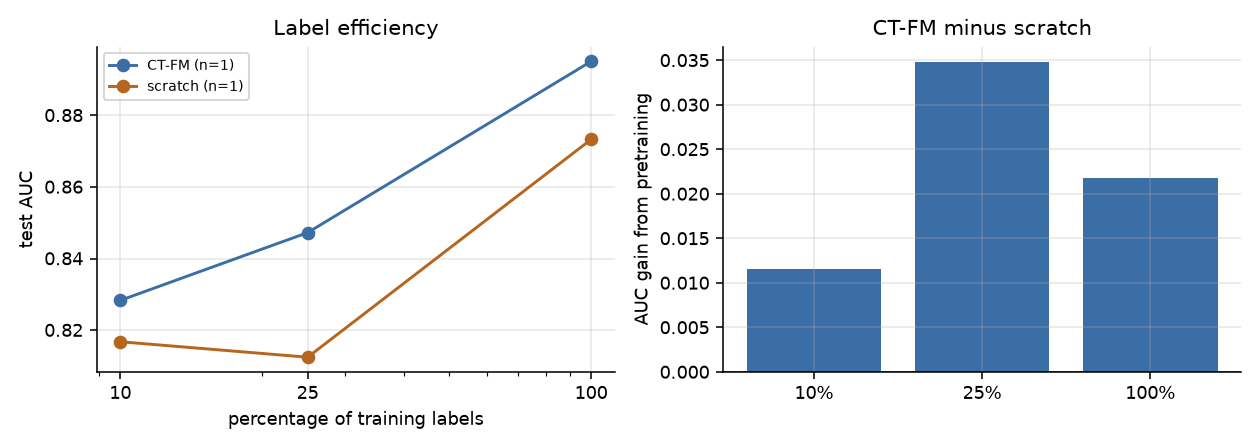
\includegraphics[width=\columnwidth]{../docs/figures/ablation.png}}
\caption{Label efficiency and the AUC gain attributable to pretraining.}
\label{fig:ablation}
\end{figure}

CT-FM initialisation wins at every budget (Table~\ref{tab:ablation},
Fig.~\ref{fig:ablation}), reaching 0.895 AUC and 0.830 balanced accuracy at full
supervision against 0.873 and 0.788 from scratch.

The caveat is material and we state it rather than bury it. A seed replicate
reversed the 10\% result, giving scratch 0.805 against CT-FM 0.802. The smallest
gain in Table~\ref{tab:ablation} therefore lies inside seed variance. The 25\%
and 100\% gains are larger and more plausible, but three or more seeds are
required before any of these numbers should be quoted as established. Running
the replicate is what exposed this, and it cost fourteen minutes.

\subsection{Calibration}

Expected calibration error under MC dropout is 0.145 with mean predictive
entropy 0.085: the model is confident and less accurate than its confidence
implies, the usual direction for a small fine-tuned network on an imbalanced
task.

\subsection{No attribution method beats random deletion}

\begin{table}[t]
\caption{Faithfulness and stability, 64 test volumes}
\label{tab:faith}
\centering
\footnotesize\begin{tabular}{lcccc}
\toprule
{\footnotesize Method} & {\footnotesize Del.$\downarrow$} & {\footnotesize Ins.$\uparrow$} & {\footnotesize AOPC$-$rnd} & {\footnotesize Stab.} \\
\midrule
Random baseline        & \textbf{0.587} & --    & --      & -- \\
LRP $\varepsilon$+flat & 0.819 & 0.972 & $-0.221$ & 0.012 \\
LRP $\varepsilon\gamma$box & 0.822 & 0.972 & $-0.224$ & $-0.015$ \\
LRP $\alpha2\beta1$    & 0.816 & 0.973 & $-0.219$ & 0.220 \\
Grad-CAM               & 0.712 & 0.974 & $-0.119$ & \textbf{0.924} \\
\bottomrule
\end{tabular}
\end{table}

\begin{figure}[t]
\centerline{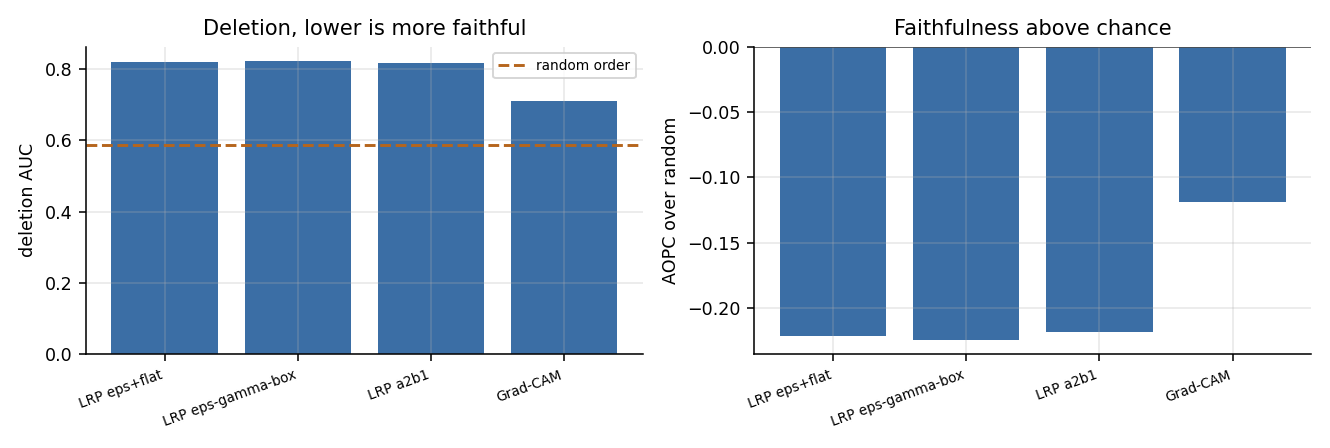
\includegraphics[width=\columnwidth]{../docs/figures/faithfulness.png}}
\caption{Deletion AUC against the random-order baseline, and AOPC relative to
random. All four attribution methods fall on the wrong side of the baseline.}
\label{fig:faith}
\end{figure}

A faithful map should sit \emph{below} the random baseline on deletion AUC. All
four sit well above it (Table~\ref{tab:faith}, Fig.~\ref{fig:faith}): removing
the voxels these methods rank highest damages the prediction \emph{less} than
removing random voxels.

We do not read this as evidence that the maps are worthless. It is a property of
the metric under volumetric masking. Random deletion scatters replaced voxels
uniformly through the volume; at 5\% this already produces something no CT
scanner would output, and the network's response collapses because the input has
left the data manifold. Attribution-guided deletion removes a compact contiguous
region, which remains a far more plausible scan. The random baseline wins by
destroying the image, not by identifying evidence.

Two consequences follow. On this task and at this scale, deletion is not a
usable adjudicator of explanation quality, and a manifold-preserving masking
scheme, such as inpainting the deleted region, is required before the protocol
can discriminate. Insertion, meanwhile, separates nothing: all four methods
recover to 0.972--0.974.

\subsection{Stability separates what deletion cannot}

Under perturbation the methods diverge sharply. Grad-CAM maps are almost
invariant (0.924) while LRP maps essentially decorrelate (0.012, $-0.015$,
0.220). This is not straightforwardly a defect of LRP. Grad-CAM is stable
\emph{because} it is coarse: a $4^3$ map upsampled to $64^3$ has little freedom
to move. LRP resolves to input resolution and pays in sensitivity. Whether a
fine-grained map that shifts under imperceptible noise is preferable to a coarse
one that does not is a genuine question that neither metric here settles.

\begin{figure}[t]
\centerline{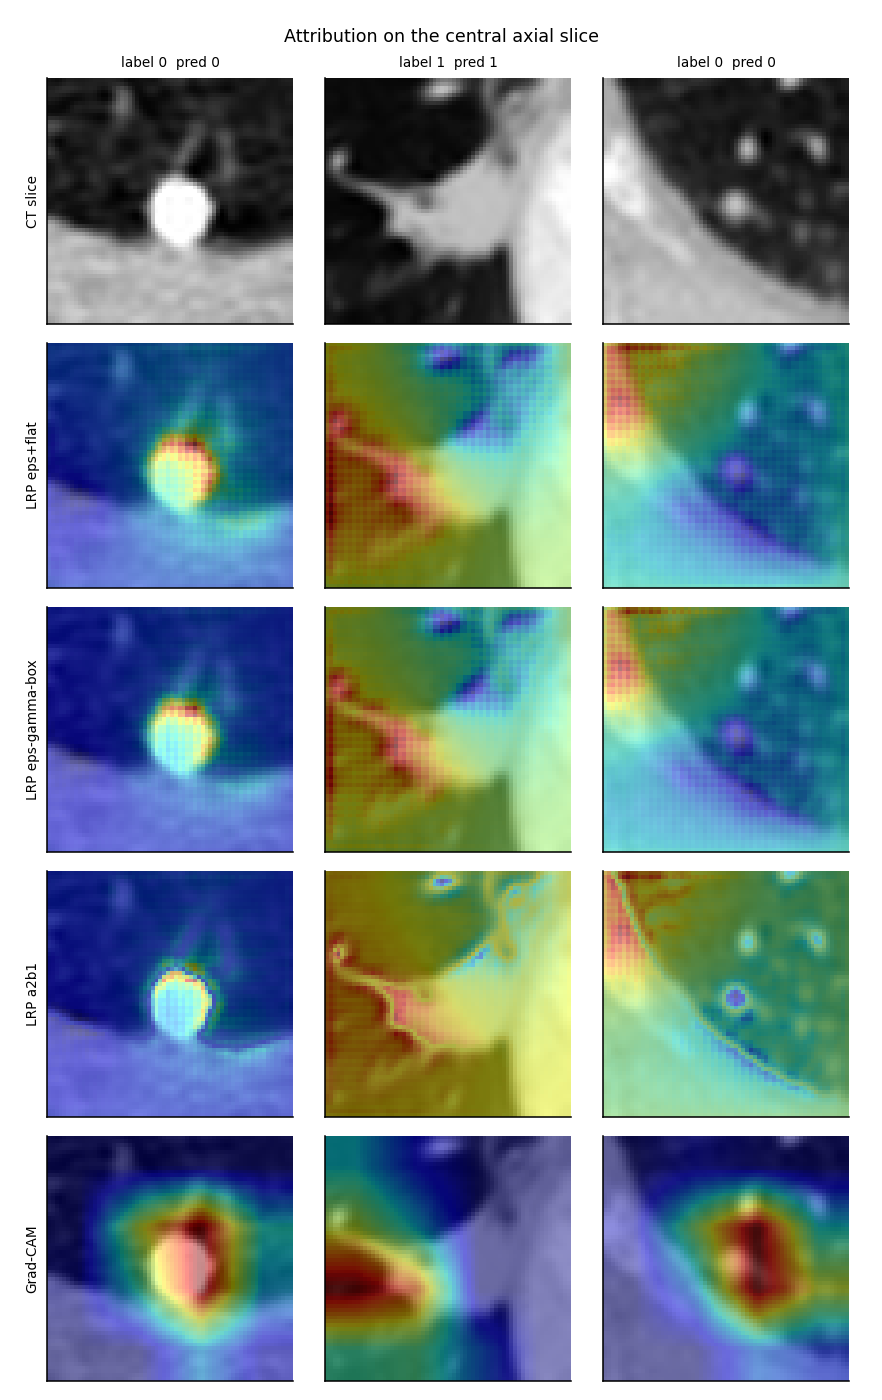
\includegraphics[width=\columnwidth]{../docs/figures/attribution_panel.png}}
\caption{Attribution on the central axial slice for three test volumes.}
\label{fig:panel}
\end{figure}

\subsection{Uncertainty against faithfulness}

\begin{figure}[t]
\centerline{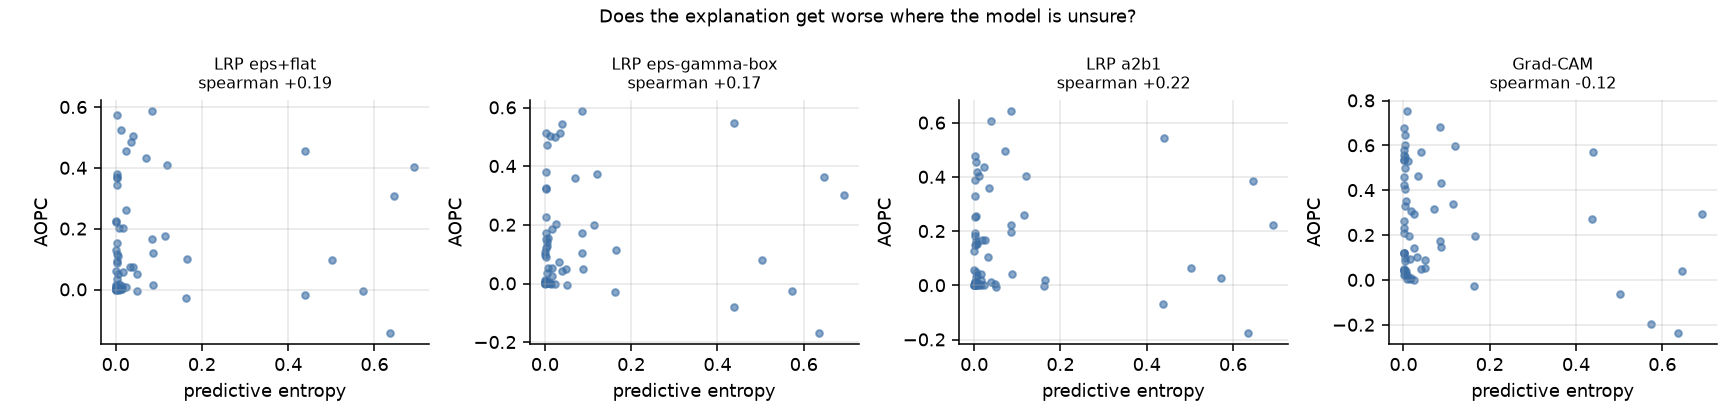
\includegraphics[width=\columnwidth]{../docs/figures/uncertainty_vs_faithfulness.png}}
\caption{Per-sample predictive entropy against AOPC. Correlations are weak and
the three LRP composites agree with one another and disagree with Grad-CAM.}
\label{fig:unc}
\end{figure}

Spearman correlations between predictive entropy and per-sample AOPC are $+0.190$,
$+0.174$ and $+0.221$ for the three LRP composites and $-0.124$ for Grad-CAM.
The LRP composites agree with each other and lean weakly positive, meaning
explanations are if anything marginally more faithful where the model is least
certain. With 64 volumes none of these is significant; the honest reading is
that the experiment is underpowered rather than that the effect is absent. The
question, posed for segmentation by Salahuddin et
al.~\cite{salahuddin2024renal}, is the right one and needs an order of magnitude
more data.

\section{Limitations}

The headline ablation uses a single seed, and the one replicate we ran already
overturned its smallest gain. The explanation analysis covers 64 volumes,
sufficient to demonstrate that the deletion metric misbehaves but not to resolve
a weak correlation. Our deletion baseline replaces voxels with the dataset mean;
a blurred or inpainted baseline stays nearer the data manifold and would likely
change the conclusion of Section~III-C, and this is the first thing we would
fix. Inputs are $64^3$ patches rather than whole chest CT, so a model pretrained
on complete scans may not be exercised as intended. Uncertainty uses MC dropout
only; deep ensembles are implemented but their members were not trained in time.

\section{Conclusion}

Self-supervised CT pretraining improved downstream nodule classification at
every label budget, with the smallest gain inside seed noise. More usefully, the
standard deletion protocol ranked every attribution method below a random
baseline, and the cause is the baseline's distribution shift rather than the
explanations' quality. Faithfulness metrics inherited from 2D natural images
require manifold-preserving masking before they can be trusted to adjudicate
explanation quality on volumetric medical data. We recommend reporting the
random control explicitly, since without it the same numbers would have read as
a straightforward endorsement of whichever method scored best.

\section*{Reproducibility}

Code, result files and all figures are available at
\url{https://github.com/Joana-Mansa/ct-fm-lrp-uncertainty}. The full ablation
runs in approximately 14 minutes on one A100. On Volta hardware, \texttt{torch}
must be pinned to 2.5.1+cu121; releases from 2.14 ship an architecture list
beginning at \texttt{sm\_75} and every CUDA call fails.

\begin{thebibliography}{00}
\bibitem{pai2025ctfm} S. Pai et al., ``Vision foundation models for computed
tomography,'' \emph{arXiv:2501.09001}, 2025.
\bibitem{bach2015lrp} S. Bach, A. Binder, G. Montavon, F. Klauschen,
K.-R. M\"uller, and W. Samek, ``On pixel-wise explanations for non-linear
classifier decisions by layer-wise relevance propagation,'' \emph{PLoS ONE},
vol. 10, no. 7, 2015.
\bibitem{anders2021zennit} C. J. Anders, D. Neumann, W. Samek, K.-R. M\"uller,
and S. Lapuschkin, ``Software for dataset-wide XAI: from local explanations to
global insights with Zennit, CoRelAy and ViRelAy,'' \emph{arXiv:2106.13200},
2021.
\bibitem{selvaraju2017gradcam} R. R. Selvaraju et al., ``Grad-CAM: visual
explanations from deep networks via gradient-based localization,'' in
\emph{ICCV}, 2017.
\bibitem{samek2017evaluating} W. Samek, A. Binder, G. Montavon, S. Lapuschkin,
and K.-R. M\"uller, ``Evaluating the visualization of what a deep neural network
has learned,'' \emph{IEEE Trans. Neural Networks and Learning Systems}, vol. 28,
no. 11, 2017.
\bibitem{salahuddin2024renal} Z. Salahuddin et al., ``Counterfactuals and
uncertainty-based explainable paradigm for the automated detection and
segmentation of renal cysts in computed tomography images: a multi-center
study,'' \emph{arXiv:2408.03789}, 2024.
\bibitem{salahuddin2022transparency} Z. Salahuddin, H. C. Woodruff,
A. Chatterjee, and P. Lambin, ``Transparency of deep neural networks for medical
image analysis: a review of interpretability methods,'' \emph{Computers in
Biology and Medicine}, vol. 140, 2022.
\bibitem{yang2023medmnist} J. Yang et al., ``MedMNIST v2: a large-scale
lightweight benchmark for 2D and 3D biomedical image classification,''
\emph{Scientific Data}, vol. 10, 2023.
\bibitem{armato2011lidc} S. G. Armato III et al., ``The Lung Image Database
Consortium (LIDC) and Image Database Resource Initiative (IDRI): a completed
reference database of lung nodules on CT scans,'' \emph{Medical Physics},
vol. 38, no. 2, 2011.
\bibitem{gal2016dropout} Y. Gal and Z. Ghahramani, ``Dropout as a Bayesian
approximation: representing model uncertainty in deep learning,'' in \emph{ICML},
2016.
\end{thebibliography}

\end{document}
